\documentclass[12pt]{article} 

%\documentclass[11pt, onecolumn]{ieeeconf}
%\linespread{1.3}

\usepackage{graphicx}
\usepackage{graphics} % for pdf, bitmapped graphics files
\usepackage{epsfig} % for postscript graphics files
%\usepackage{mathptmx} % assumes new font selection scheme installed
\usepackage{times} % assumes new font selection scheme installed
\usepackage{amsmath} % assumes amsmath package installed
\usepackage{amssymb}  % assumes amsmath package installed
\usepackage{bm}  % assumes amsmath package installed
\usepackage{enumerate}  % assumes amsmath package installed



\def\bs{\boldsymbol}
\def\mb{\mathbb}
\def\cw{3.45in}
\def\ts{\textsuperscript}
\newcommand{\norm}[1]{\lVert#1\rVert}

\title{Peregrine: help}

%%% first author
\author{Sachit Butail}

\date{}


\begin{document}

\maketitle
\thispagestyle{empty}
\pagestyle{empty}

%%%%%%%%%%%%%%%%%%%%%%%%%%%%%%%%%%%%%%%%%%%%%%%%%%%%%%%%%%%%%%%%%%%%%%
%\begin{abstract}
%Peregrine is an automated tracking system for studying collective animal behavior. 
%\end{abstract}


%%%%%%%%%%%%%%%%%%%%%%%%%%%%%%%%%%%%%%%%%%%%%%%%%%%%%%%%%%%%%%%%%%%%%%
\section{Introduction}
The technical details for the methods used in peregrine are described in detail in the following papers \cite{Butail2011,Butail2012b,Butail2012c, Butail2013c}. In particular, two-dimensional position tracking draws from \cite{Butail2013c, Butail2012b}, and shape tracking draws from \cite{Butail2011,Butail2012c}. Modifications to these approaches, if any, are described here.

\begin{figure}[ht]
\centering
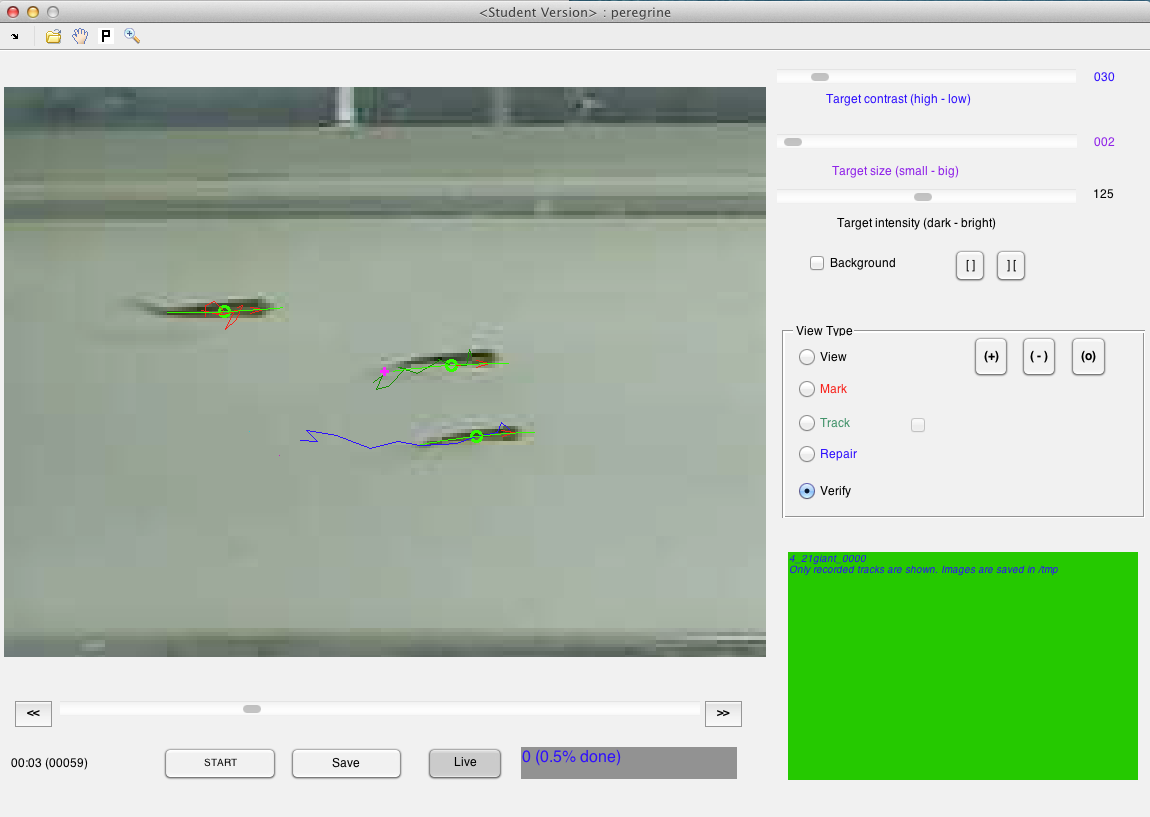
\includegraphics[width=.995\linewidth]{screenshot}
\caption{Tracking shape and orientation of three fish in a flow tank. Two fish on the top are occluded}
\label{fig:sample_tracks}
\end{figure}

\begin{figure}[ht]
\centering
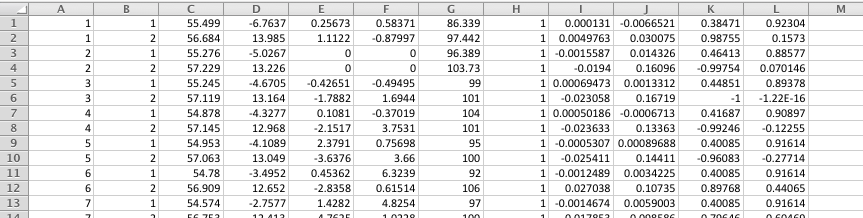
\includegraphics[width=.495\linewidth]{output}
\caption{Output of the tracker is stored in a csv file where each column corresponds to a single frame and a single target.}
\label{fig:output}
\end{figure}

\section{Preferences and initial setup}
\begin{figure}[h]
\centering
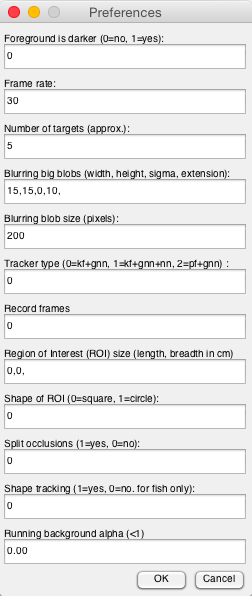
\includegraphics[width=.495\linewidth]{prefs}
\caption{Preferences}
\label{fig:prefs}
\end{figure}

\section{Tracking}

\subsection{Position and velocity tracking}
Position and velocity tracking uses a Kalman filter \cite{BarShalom1987}, and global data-association \cite{Kuhn1955} to track multiple targets in a video. The output csv file is ordered as: frame, target-id, horizontal-coordinate, vertical-coordinate, horizontal-velocity, vertical-velocity, size-in-pixels 

\subsection{Shape tracking}
\begin{itemize}
\item Find the centroid
\item Optimize on orientation ($\theta$) and parabola fit to minimize the least squares error in the body frame
\item Feed the measurements to a particle filter
\end{itemize}


\subsection{Repair mode}
The repair mode allows the user to fix the tracks by
\begin{enumerate}
\item Stitch broken tracks
\item Switch tracks before and after an occlusion that was not resolved properly
\item Add a new point for an undetected target
\end{enumerate}

\subsection{Command line mode}
\emph{pg\_cmd}
\section{Global observations}

Once trajectory data is available, the command \emph{get\_obs} computes the  various measures of collective behavior. We assume that both position and velocity of each target (for example fish) is available at all times during the experiment. We also assume that the each fish identified by a unique number that can be used to quantify the behavior during the trial. Unless specified, we make the assumption that the heading is the same as the direction of motion. (This assumption is dropped, for example, when the fish are in a water tunnel.)

\begin{enumerate}
\item \emph{Group cohesion:} The degree of cohesion in groups is described in terms of the average nearest-neighbor distance (ANND) \cite{Webster2007, Kolpas2008}. Given the two-dimensional position $\bs{r}_i[k]$ of the $i$-th fish at frame $k$, the ANND during that frame is \cite{Kolpas2008}
\begin{equation}
\mathrm{ANND}[k]=\frac{1}{N}\sum_{i=1}^N\min_{j\in \{1,\ldots,N\}, j\ne i}(\norm{\bs{r}_i[k]-\bs{r}_j[k]}),
\end{equation}
where $N$ is the total number of fish and $\norm{\cdot}$ denotes the standard Euclidean norm. 
\item \emph{Group coordination:} is captured through the polarization (Pol) that measures the degree of alignment between the directions of motion of the fish \cite{Vicsek1995}. Given the two-dimensional velocity $\bs{v}_i[k]$ of the $i$-th fish at frame $k$, the polarization at that frame is
\begin{equation}
\mathrm{Pol}[k]=\frac{1}{N}\Big\|\sum_{i=1}^N\hat{\bs{v}}_i[k]\Big\|, 
\end{equation} 
where $\hat{\bs{v}}_i[k] =\frac{\bs{v}_i[k]}{\norm{\bs{v}_i[k]}}$ is the direction of motion. 
\item \emph{Group speed:} is computed to describe average speed of the subjects, and is  given by 
\begin{equation}
S[k]=\frac{1}{N}\sum_{i=1}^N\|\bs{v}_i[k]\|
\end{equation}
\item \emph{Group angular momentum}: the normalized group angular momentum $\hat{L}$ is indicative of milling patterns \cite{Chuang2007, Couzin2003a}, with $\hat{L}=1$ for single milling formations and  $\hat{L}=0$ for a coherent one-directional formation \cite{Chuang2007}. Depending on how $\bs{r}_i$ is defined, the angular momentum can be computed about the group center of mass \cite{Aureli2012}, or about the center of the observation region.
\begin{equation}
\hat{L}[k]=\frac{\|\sum_{i=1}^N\bs{r}_i[k]\times\bs{v}_i[k]\|}{\sum_{i=1}^N\|\bs{r}_i[k]\|\|\bs{v}_i[k]\|}
\end{equation}
\item \emph{Group interaction:} with a focal fish (or an external stimulus such as a robot) is quantified in terms of values such as distance, alignment and relative speed. We denote the focal fish or target index with a subscript $\bs{r}_f$. Specifically the observables are
	\begin{enumerate}
		\item \emph{Average distance to the focal fish:} Average distance of all other fish to the focal fish
		\begin{equation}
			\hat{d}[k]=\frac{1}{N-1}\sum_{i\in\{1,\ldots,N\}, i\ne f}\|\bs{r}_i[k]-\bs{r}_f[k]\|
		\end{equation}
		\item \emph{Minimum distance to the focal fish:} Minimum distance to the focal fish between all other fish
		\begin{equation}
		\tilde{d}[k]=\underset{i\in\{1,\ldots,N\}, i\ne f}{\operatorname{argmin}}\|\bs{r}_i[k]-\bs{r}_f[k]\|
		\end{equation}
		\item \emph{Group relative speed with respect to the focal fish:}
		\begin{equation}
		\tilde{S}[k]=\Big(\frac{1}{N-1}\sum_{i\in\{1,\ldots,N\}, i\ne f}\|\bs{v}_i[k]\|\Big)-\|\bs{v}_f[k]\|
		\end{equation}
		\item \emph{Alignment to the focal fish:}
	\end{enumerate}
\item \emph{Group behavior:} quantifies on an average the behavior of subjects such as percentage time spent freezing, thrashing, or swimming. These values allow us to determine if the subjects were in general scared or not. The specific observables are:
	\begin{enumerate}
		\item \emph{Time spent freezing:} To elucidate the behavior of the subjects, we score the time spent freezing during each trial. This value is computed automatically based on the condition that a fish is considered freezing during a frame if it spends two continuous seconds within a ball of radius of 2 cm \cite{Kopman2013}. Freezing is recorded if at least one fish satisfied this condition.
		\item \emph{Excursions of focal from shoal:} To measure the number of excursions from the shoal of a particular fish, we use the definition of shoal membership as described in \cite{Miller2011a}. In particular, we (i) compute the time series of average nearest neighbor distance of the focal fish,(ii) distribution of ANND for all fish over all frames is computed. Use the mode of this distribution as the threshold, divide the time series into segments where the individual's ANND goes above the mode, and (iii) find the distribution of the maximum ANND of each segment. The upper p=0.05 quantile of the max ANND distribution determines if a segment is an excursion or not. 
	\end{enumerate}
\end{enumerate}


%%%%%%%%%%%%%%%%%%%%%%%%%%%%%%%%%%%%%%%%%%%%%%%%%%%%%%%%%%%%%%%%%%%%%%
\section{Acknowledgement}
The authors would like to acknowledge assistance from Dynamical Systems Laboratory, Polytechnic Institute of New York University, and Collective Dynamics and Control Laboratory, University of Maryland.


\bibliographystyle{unsrt}
\bibliography{$HOME/Documents/refs/library}
\end{document}
